\chapter{Introduction to GPU programming}
\label{chap:gpu_intro}


Graphics Processing Units (GPUs) have evolved from specialized hardware designed solely for rendering graphics to powerful, general-purpose processors capable of handling complex computations. In the early years, 3D acceleration carts, as they used to be called, were devoted to offloading the rendering tasks, such as drawing pixels, filling polygons with textures, or computing geometry, from the CPU~\cite{pratx2011gpu}. And because processing pixels is inherently parallel, GPU architectures were being developed with different paradigms compared to ordinary CPUs. GPU chip semantics is oriented on high performance achieved by immense parallelism, with a design that promotes further scalability. Its die surface is largely occupied by compute cores with very little space dedicated to cache and control, which contradicts the CPU design (the graphical reference depicted in Figure~\ref{fig:cpu-gpu}). Thus, GPUs can be much more powerful than CPUs if the solution is carefully designed for it~\cite{navarro2014survey}.

The shift from specialized graphics processing to general-purpose computing was marked by the introduction of programming frameworks such as CUDA (Compute Unified Device Architecture) by NVIDIA and OpenCL (Open Computing Language) by Khronos group. As extensions to C/C++, these frameworks simplified the process of writing code for GPU and streamlined the adoption of GPU for general-purpose programming~\cite{croix2009introduction}. CUDA, in particular, has become the de facto standard for GPU programming due to its ease of use, performance, and wide adoption in the scientific community.

In this chapter, we provide an overview of the GPU hardware architecture and the CUDA programming model. We also discuss the main optimization techniques used in GPU programming, which are essential for achieving high performance on GPUs. The knowledge presented in this chapter serves as a foundation for the subsequent chapters, where we detail the GPU optimizations of scientific algorithms and describe the parallelization use-cases of the Noarr library.

\section{GPU Hardware Architecture and Programming Model}
\label{sec:gpu_arch}

Generally, a programming model serves as a high-level abstraction of the hardware architecture, allowing programmers to write code that can run and scale well without prior knowledge of the underlying hardware specifics. The terminology within the model varies depending on the programming framework or GPU vendor, but the core concepts remain the same. To maintain conciseness, we continue with the description in CUDA terms.

Let us start with the hardware. The main building block of a GPU is the \emph{Streaming Multiprocessor} (SM). The diagram in Figure~\ref{fig:sm} displays its composition: SM couples hundreds of compute cores, a register file, L1 cache also called \emph{shared memory}, and schedulers responsible for independent scheduling of groups of threads. There are multiple SMs in a GPU, their number highly correlating with a GPU cost --- the more high-end the GPU, the more SMs it holds. All SMs are connected via a high-speed interconnect to the GPU RAM, the \emph{global memory}.

\begin{figure}[h]
	\centering
	\begin{minipage}{.5\textwidth}
        \centering
        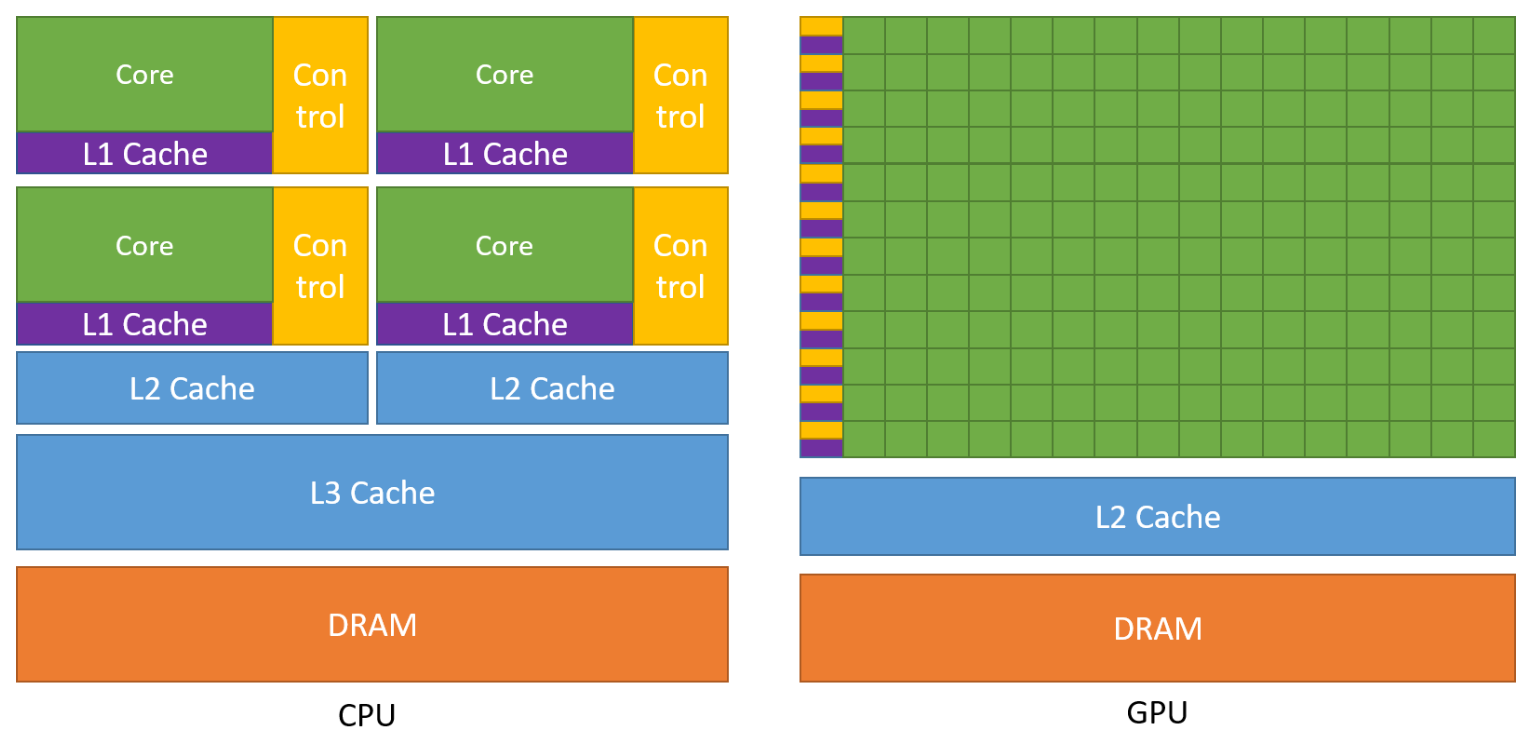
\includegraphics[width=\textwidth]{img/cpu-gpu}
        \caption{Comparison of CPU and GPU chip design~\cite{site:cuda}.}
        \label{fig:cpu-gpu}
	\end{minipage}%
	\begin{minipage}{.5\textwidth}
        \centering
        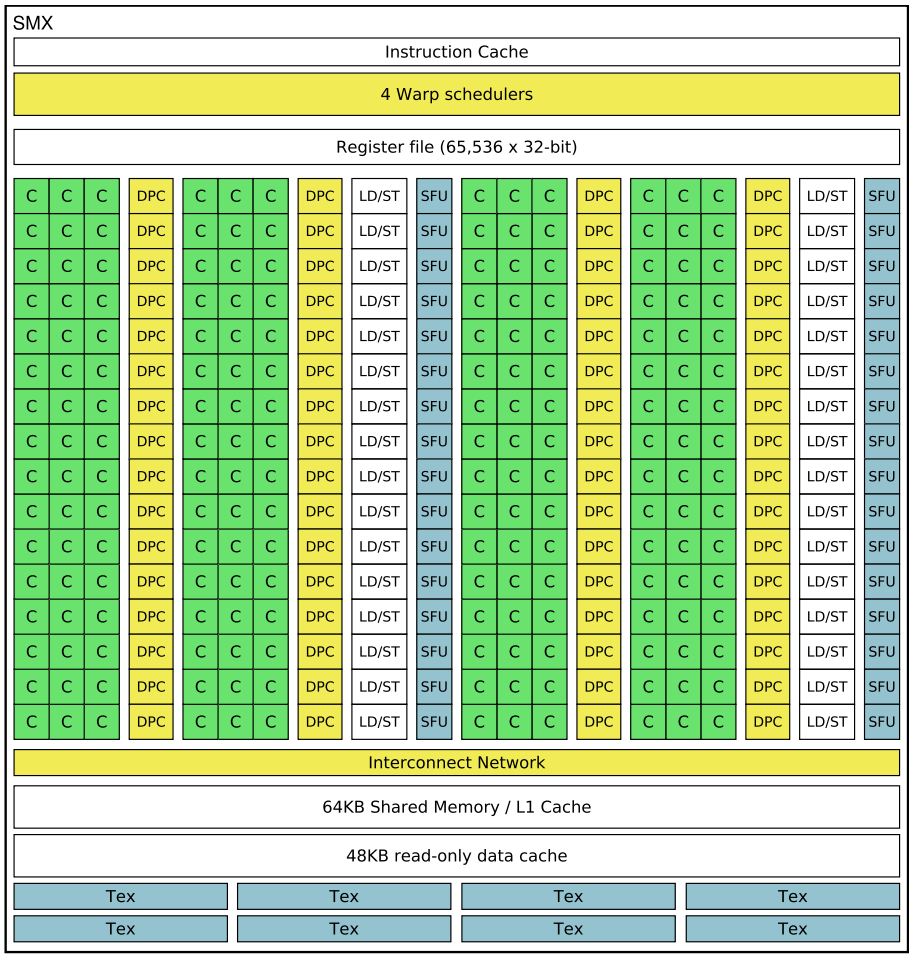
\includegraphics[width=0.8\textwidth]{img/sm}
        \caption{Diagram of a streaming multiprocessor~\cite{navarro2014survey}.}
        \label{fig:sm}
	\end{minipage}
\end{figure}

The abstraction of this highly parallel architecture is based on organizing threads into hierarchical levels. The basic units of execution are \emph{threads}. These are organized into \emph{blocks}, groups of threads \emph{executed on the same SM}, sharing a register file and the shared memory. Lastly, a group of blocks that is executed independently on multiple SMs is called a \emph{grid}. Thus, the grid, as depicted in Figure~\ref{fig:grid}, defines the amount (and dimensionality) of concurrent work to be done on a GPU. Figure~\ref{fig:grid-sm} shows how the hierarchy of threads maps to GPU hardware, abstracting away the details of the hardware architecture in the process.

\begin{figure}
	\centering
	\begin{subfigure}{.5\textwidth}
		\centering
        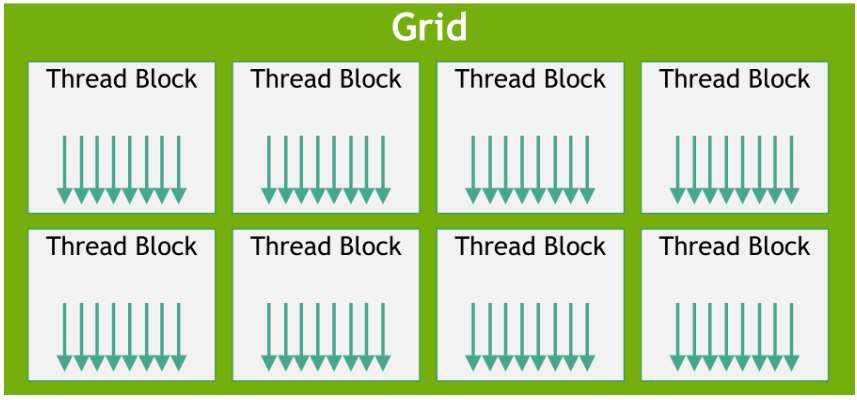
\includegraphics[width=0.8\textwidth]{img/grid}
        \caption{GPU grid of $8$ blocks organized in $2\times4$ fashion, each block consisting of $8$ threads.}
        \label{fig:grid}
	\end{subfigure}%
	\begin{subfigure}{.5\textwidth}
		\centering
        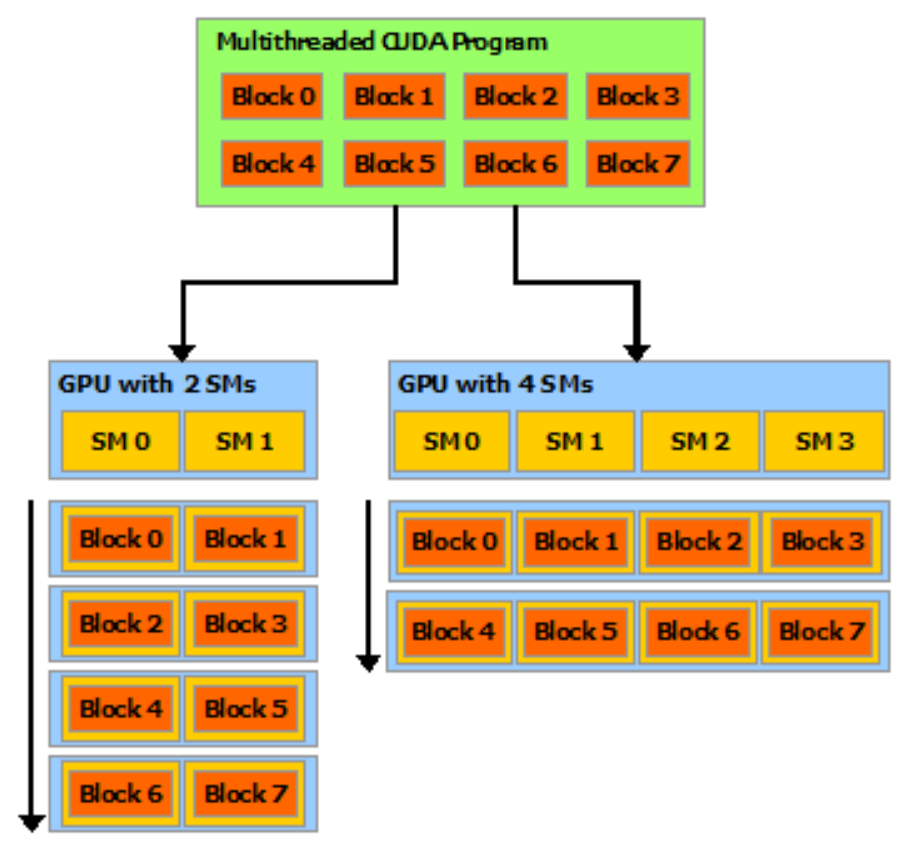
\includegraphics[width=0.7\textwidth]{img/grid-sm}
        \caption{The assignment of blocks in a grid to SMs on GPUs with various SM counts.}
        \label{fig:grid-sm}
	\end{subfigure}
    \caption{A diagram of a grid ands its SMs assignment~\cite{site:cuda}.}
\end{figure}

Conceptually, this programming model is based on \emph{Single Instruction, Multiple Data} (SIMD) architecture, which is a type of parallel processing where a single instruction is executed on multiple data streams. In practice, SM issues threads in groups of $32$, called \emph{warps}, which execute in \emph{lockstep} --- all performing the same instruction at once. A more accurate description of this type of processing is \emph{Single Instruction, Multiple Threads} (SIMT), which is nowadays used to describe the GPU programming model.

As a consequence of SIMT architecture and lockstep execution, GPUs favor \emph{data-parallel problems}. These are problems such that their solution requires applying the same function to its whole domain (e.g., an $n$-dimensional array). The data-parallel problems are well-suited for GPUs, as they allow all threads to execute \emph{the same instruction} but on \emph{different data}~\cite{navarro2014survey}.

\section{Optimizing for GPU performance}
\label{sec:gpu_optim}

Contemporary GPU devices are becoming increasingly sophisticated and are equipped with a variety of control-flow mechanisms, interthread communication, atomic instruction, and others, which allow for a broader range of problems to be solved on GPUs. However, applying these features correctly is not trivial, as it requires a deep understanding of the architecture and programming model. Thus, achieving optimal performance on a GPU requires careful consideration of various aspects. Let us detail the most important ones to watch for when optimizing GPU code~\cite{pratx2011gpu}.

\subsection{Arithmetic intensity}
\label{sec:arithmetic_int}

The peak performance of contemporary high-end GPUs is nowadays measured in TFLOPS (trillions of floating-point operations per second). In order to determine an actual achievable performance of a program, memory bandwidth needs to be considered virtually always. Comparing peak performance and memory bandwidth of current GPUs, we quickly conclude that the cores can not be fed data at the same rate as they can compute.

Therefore, one of the most important constants in GPU programming is \emph{ops-per-byte} ratio. It is computed as the ratio of math and memory bandwidth, and it simply determines how many math operations per transferred byte must be executed to achieve the theoretical maximum performance. For example, NVIDIA V100 GPU achieves $14$ TFLOPS peak single-precision performance with a memory bandwidth of $900$ GB/s. This results $\frac{14}{0.9} \approx 15$ ops-per-byte ratio. As a simple rule of thumb, a program that performs less than $60$ single-precision floating point operations per single $4$-byte load/store will be \emph{memory-bound} and a program that performs more operations will be \emph{compute-bound}. Such a property of a program is called \emph{arithmetic intensity} and is a key factor in determining the performance of a GPU kernel.

To get more detail in hardware utilization than just comparing ops-per-byte ratio with arithmetic intensity, modern profilers include the \emph{roofline model}~\cite{williams2009roofline}. It is a graphical representation of a hardware attainable performance, given the algorithm arithmetic intensity. Figure~\ref{fig:roof} shows an example of a roofline diagram, where the x and y axes represent the arithmetic intensity and the performance, respectively. The horizontal lines represent the achievable performance of single- and double-precision floating-point operations and the diagonal line represents the memory bandwidth. The roofline model can be used to determine the performance bottlenecks of a program and to guide optimization efforts.

\begin{figure}
    \centering
    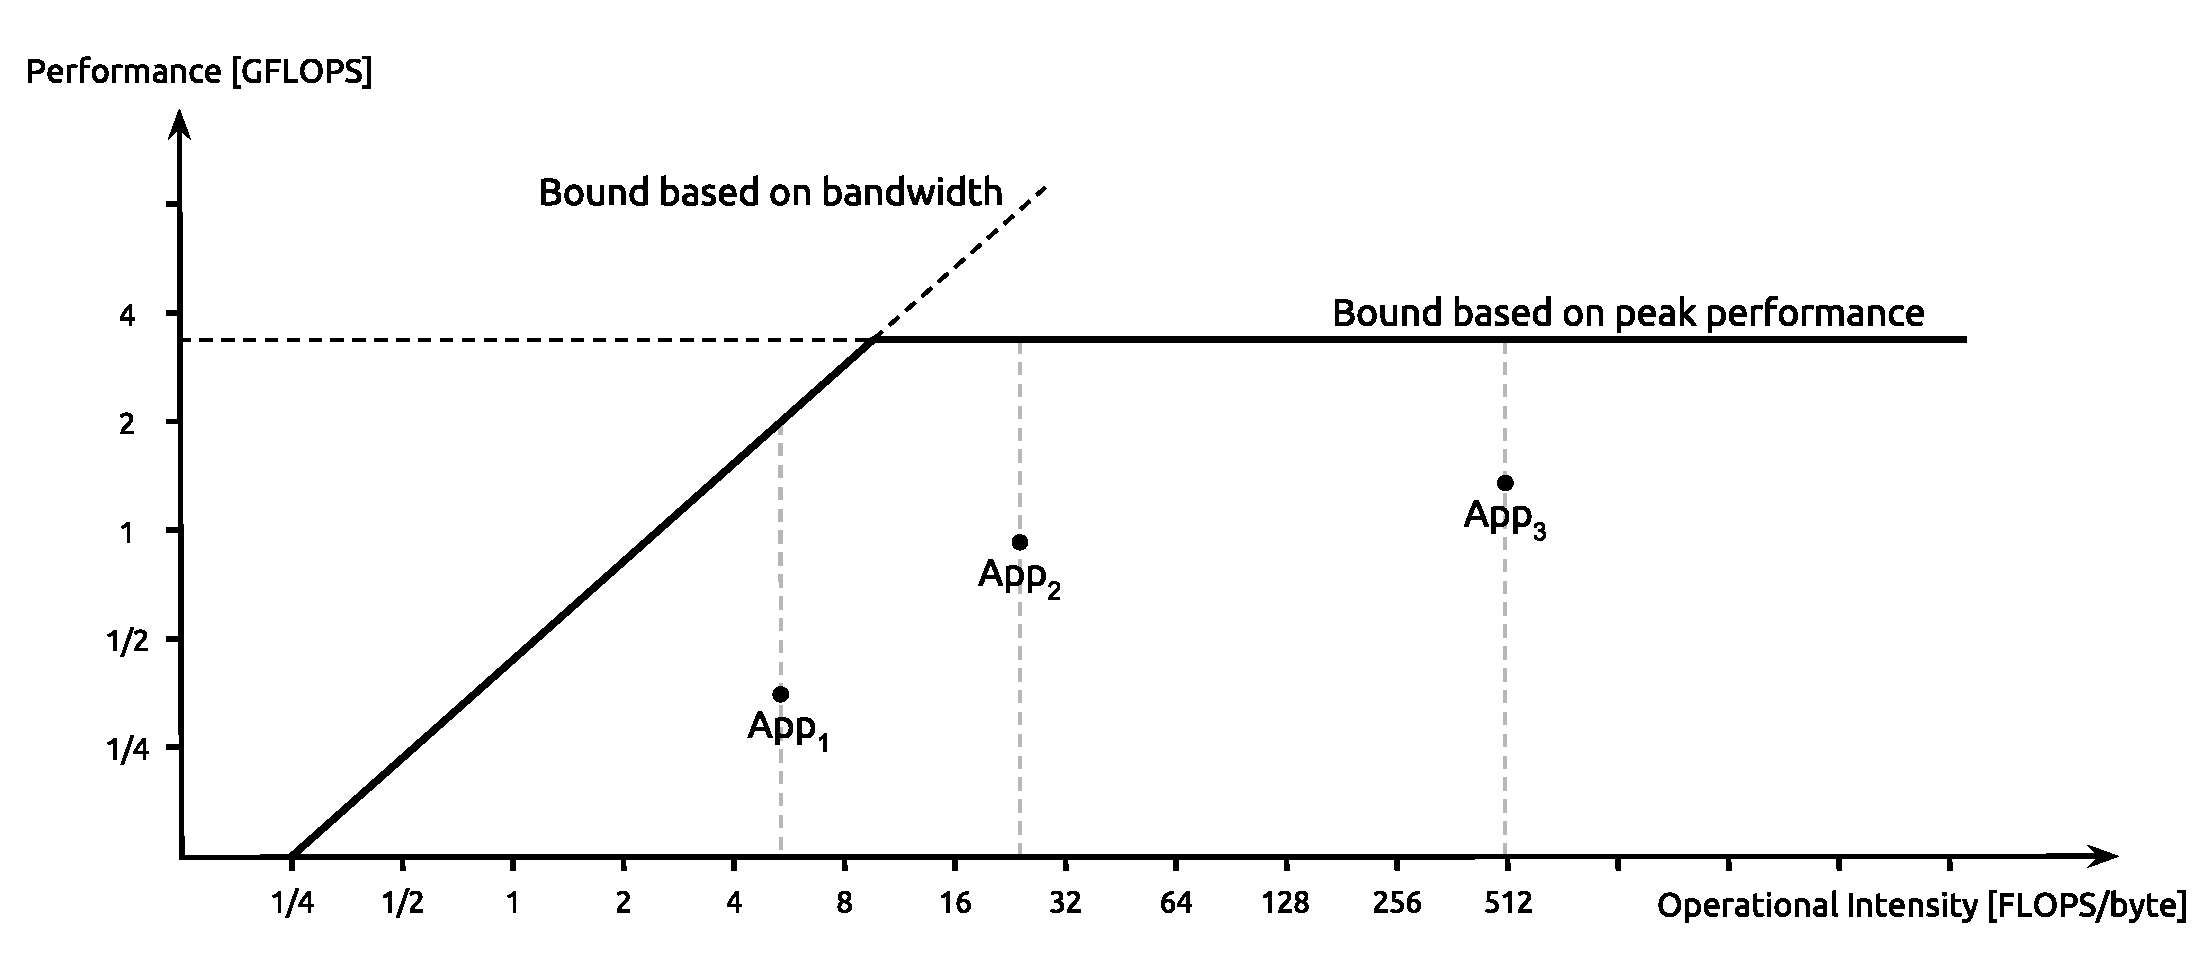
\includegraphics[width=0.8\textwidth]{img/Example_of_a_Roofline_model.pdf}
    \caption{The example of a roofline diagram~\cite{wiki:Roofline_model}. The x axis denotes arithmetic intensity (also called operational intensity) and y axis shows attainable performance.}
    \label{fig:roof}
\end{figure}

Strictly speaking, there are two ways how to decrease the gap between arithmetic intensity and ops-per-byte ratio: If a program allows, its operation may be reordered such that fetching the same data multiple times is avoided, promoting \emph{data reuse}, which in turn increases the arithmetic intensity. Another way is to decrease the ops-per-byte ratio by utilizing the GPU memory hierarchy, which we discuss in the following paragraphs.

\subsection{Memory hierarchy}
\label{sec:memory_hier}

A GPU thread hierarchy is accompanied by \emph{memory hierarchy}. As alluded in the previous paragraph, global off-chip memory has the highest latency and the lowest bandwidth. To avoid thread stalls measured in hundreds of cycles due to fetching data from global memory, other levels of memory hierarchies should be utilized. This process is generally called \emph{caching} but can be also interpreted as \emph{data sharing}, as the data is shared among threads in the same thread hierarchy.

Depending on the desired level of data sharing within the thread hierarchy, programmers can use various types of memory (as depicted in Figure~\ref{fig:mem-hierarchy}). On a block level, on-chip shared memory can be accessed with a magnitude lower latency and higher bandwidth than global memory. In extreme data sharing cases, threads in the same warp can use the register file as a cache with close-to-zero zero latency. However, the higher the proximity of the specific memory type to the compute cores, the lower capacity it carries. Contemporary GPUs encompass $64$k of $32$B registers, $100-200$ kB of shared memory, and $8-16$ GB of global memory for consumer-grade GPUs and up to $80$ GB for the highest-end datacenter-grade GPUs.

To sum up, the key to achieving high performance on a GPU is to minimize global memory accesses by smartly dividing the work in a thread hierarchy such that faster memory levels are utilized. Moreover, since the ops-per-byte ratio is inversely proportional to the memory bandwidth, a program using shared memory or registers as caches does not carry such significant requirements on arithmetic intensity to achieve maximum performance.

\begin{figure}
    \centering
    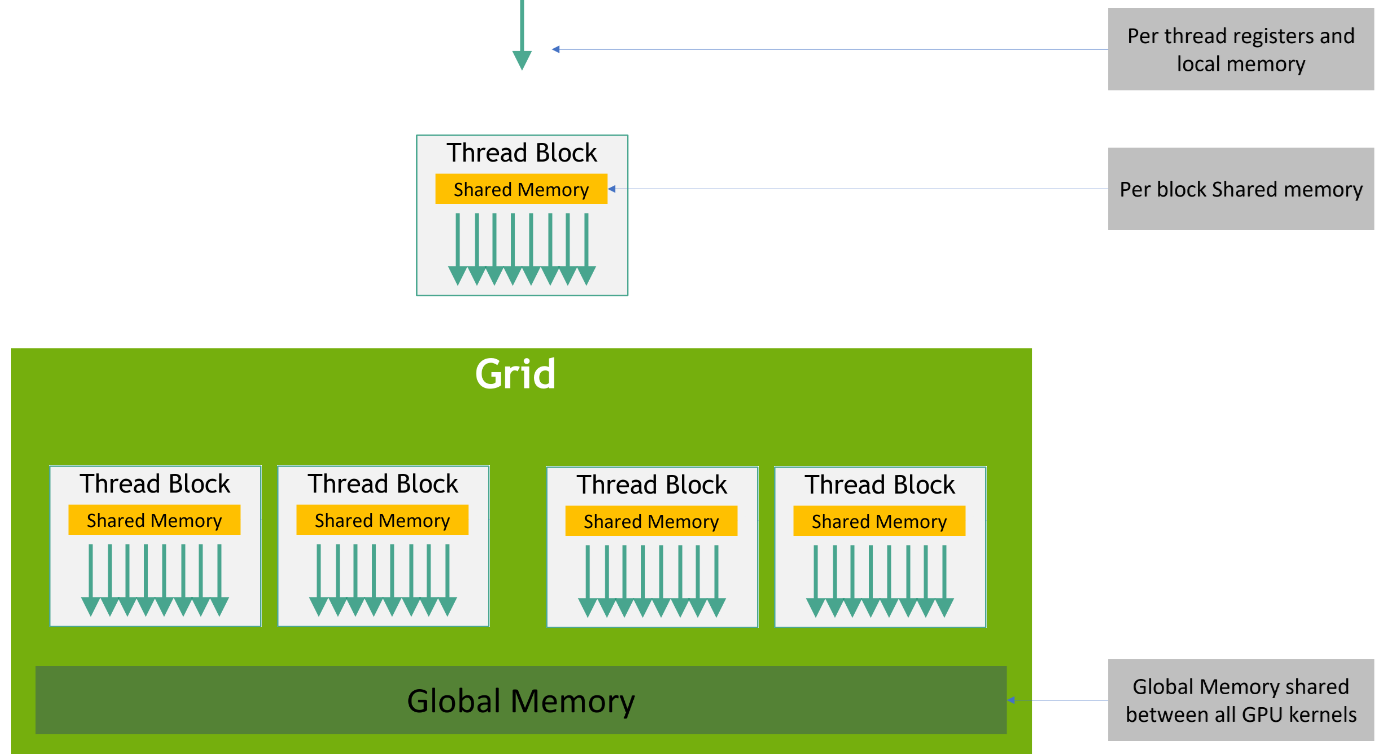
\includegraphics[width=0.6\textwidth]{img/mem-hierarchy-2.png}
    \caption{A thread hierarchy of GPU (left) and its corresponding memory hierarchy (right)~\cite{site:cuda}.}
    \label{fig:mem-hierarchy}
\end{figure}

\subsection{Memory coalescing}
\label{sec:coalescing}

Fetching data from global memory is serviced in up to $128$B wide transactions. If threads in a warp request a single byte, the GPU will fetch the whole transaction chunk, wasting the memory bandwidth on data that will never be used and negatively impacting the ops-per-byte ratio. To utilize the memory bandwidth fully, the aggregated memory accesses in a lockstep should coalesce into continuous memory locations. Figure~\ref{fig:coal} illustrates this concept.

In practice, whether memory is transferred in an optimal number of transactions is directly influenced by the layout of the data structures in use. One example may include using a column-major layout for the right-hand side matrix in matrix multiplication or avoiding the usage of linked lists.

\begin{figure}[b]
	\centering
	\begin{minipage}{.5\textwidth}
        \centering
        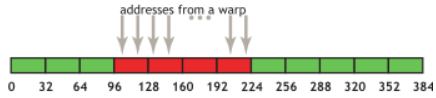
\includegraphics[width=0.9\textwidth]{img/coal1}
        \caption{Warp accesses coalesced into 4 memory transactions~\cite{site:cuda}.}
        \label{fig:coal}
	\end{minipage}%
	\begin{minipage}{.5\textwidth}
        \centering
        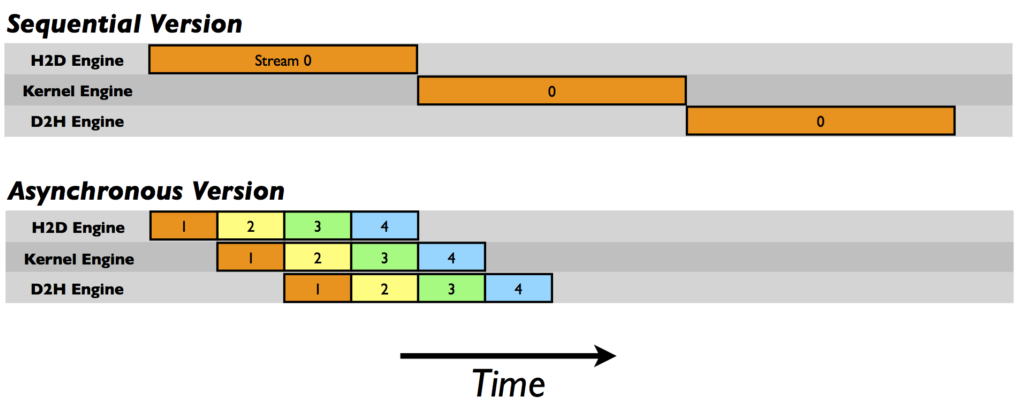
\includegraphics[width=\textwidth]{img/C2050Timeline-1024x670.png}
        \caption{Time diagram of non-overlapped (top) and overlapped (bottom) transfer and computation~\cite{site:stream}.}
        \label{fig:transfer}
	\end{minipage}
\end{figure}

\subsection{CPU--GPU data transfers}
\label{sec:transfers}

Transferring data between CPU and GPU memory spaces can pose a significant bottleneck when developing GPU programs. Usually, the interconnect which is used to transfer data between the CPU and the GPU has a much lower bandwidth even than the GPU global memory. Therefore, it is essential to avoid redundant data transfers between the host and the device.

In true data-parallel algorithms, this is generally not a big issue because these data transfers can be overlapped with computation. Such overlapping is possible by GPU \emph{task queues}, which allow the execution of multiple programs as well as CPU--GPU memory transfers in parallel. This hardware feature is exposed by the software abstraction called \emph{streams}. Figure~\ref{fig:transfer} show the ideal scenario, where one would use multiple streams to overlap three main operations always present when programming on GPUs: transferring input from CPU to GPU, GPU computation, and transferring output back from GPU to CPU.

\subsection{Thread divergence}
\label{sec:divergence}

The downside of the highly parallel SIMT architecture is handling diverging execution paths in the code. If threads in a warp take different \texttt{if} or their iteration count over a \texttt{while} loop does not match, the execution of these diverging paths will be serialized, as depicted in Figure~\ref{fig:divergence}.

Intra-warp branching should be avoided to keep the number of active threads high for the longest amount of time. Divergence can be mitigated by lifting the branching to the inter-warp level, replacing branches with arithmetic operations if possible, or unrolling warp-wise loops.

\begin{figure}
    \centering
    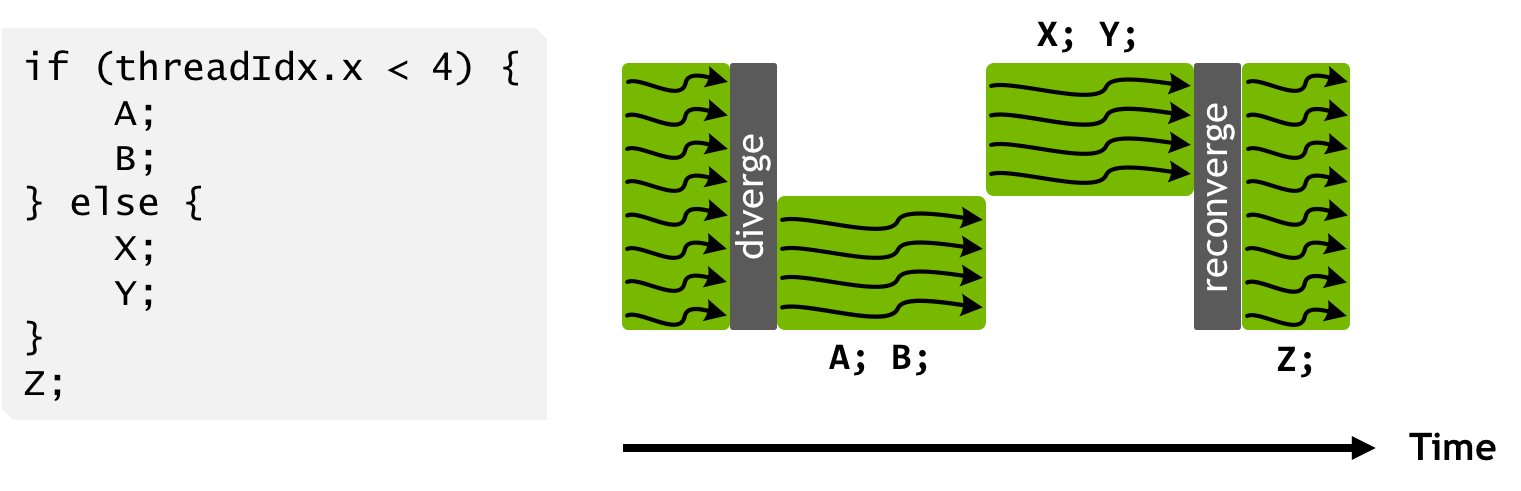
\includegraphics[width=0.8\textwidth]{img/divergence.png}
    \caption{An example of diverging code with a diagram of how warp threads would be scheduled~\cite{site:volta}.}
    \label{fig:divergence}
\end{figure}

\subsection{Thread occupancy}
\label{sec:occupancy}

The GPU is designed to run thousands of threads in parallel and tens of thousands of threads concurrently. Increasing the number of concurrent threads above the limit of compute cores is crucial for GPU utilization as it allows \emph{hiding memory latencies} by switching between active threads. A single SM can accommodate thousands of concurrent threads, although the number of accommodable cores is a magnitude lower. The SM takes advantage of this high discrepancy to aggressively context switch between different warps when the currently scheduled ones are waiting for a latency. Since all the thread contexts reside on-chip, the context switch has negligible overhead, and, provided there are enough available concurrent threads, it can effectively hide the memory latencies.

The number of concurrent threads per SM is called the \emph{thread occupancy}. It denotes the ratio of active threads to the maximum number of threads that can be executed concurrently on an SM. This metric is influenced by the resource requirements of a program: Increasing the shared memory usage per block or register usage per thread decreases the thread occupancy, which in turn decreases the parallel capacity of the GPU device.

However, a GPU code that achieves high thread occupancy uses less on-chip resources, so it is required to use slower global memory more often, which in turn decreases the computational efficiency of a thread. Thus, thread occupancy and thread efficiency compete with each other, and their optimal ratio for a given hardware should be finely tuned to achieve the best performance.

\section{Summary}

These are a few of the most dominant optimization techniques used in GPU programming. For the past few years, GPU hardware has evolved extraordinarily rapidly to satisfy the demand for hardware that can train artificial intelligence models with billions of parameters. This has brought many new features, making the device more versatile and powerful. Let it be more advanced SMs, independent thread scheduling, \emph{block cluster}, which brings a new element in the thread and memory hierarchy, specialized matrix multiplication-optimized \emph{tensor cores}, which increase ops-per-byte ratio ten-fold, or \emph{tensor memory access}, which allow asynchronous copying of non-sequential data efficiently, \dots

In summary, the field of GPU programming is vast, and optimization techniques are often intertwined and compete with each other. The optimal solution is usually a compromise between the techniques, which is highly dependent on the specific properties of the problem. In the following chapter, we will describe our work of porting scientific algorithms to GPUs using the terminology and knowledge established in this section as guidelines to detail the main optimization challenges for each of them.